\documentclass[a4paper,12pt]{article}

\usepackage[utf8]{inputenc}
\usepackage[ngerman]{babel}
\usepackage{amsmath,amssymb}
\usepackage{graphicx}
\usepackage[a4paper, left=2cm, right=3cm, bottom=2cm]{geometry}
\usepackage{fancyhdr}
\usepackage{qrcode}
\usepackage{hyperref}
\usepackage{breakurl}
\usepackage{imakeidx}
\usepackage{wrapfig}

\graphicspath{ {./images/} }

\title{Die Atombombe}
\author{Tim, Olli, Jakub}
\date{\today}

\begin{document}
\pagestyle{fancy}

\fancyfoot[LE,RO]{\thepage}
\fancyfoot[LO,CE]{Tim, Olli, J. Z.}
\fancyfoot[CO,RE]{Atombombe}

\maketitle

\begin{abstract}
nn
\end{abstract}

\newpage

\tableofcontents

\newpage

\section{Einführiung}
Die Entwicklung und der Einsatz von Atombomben im 20. Jahrhundert haben die Menschheitsgeschichte nachhaltig geprägt. Eine Atombombe basiert auf der Nutzung der enormen Energie, die bei der Kernspaltung freigesetzt wird. Im Zentrum steht die Erzeugung einer Kettenreaktion, bei der Atomkerne gespalten und dabei gewaltige Mengen an Energie in Form von Wärme, Strahlung und Druckwellen freigesetzt werden.
Zur Zündung einer Atombombe muss eine sogenannte kritische Masse erreicht werden. Dies ist die Mindestmasse an spaltbarem Material, bei der die Kettenreaktion selbstständig und unkontrolliert abläuft. Zwei Hauptmethoden zur Erreichung der kritischen Masse wurden entwickelt: das Gun-Design und das Implosions-Design.

\section{Aufbau}
\begin{wrapfigure}{r}{0.4\textwidth}
    \vspace{-1cm}
    \centering
    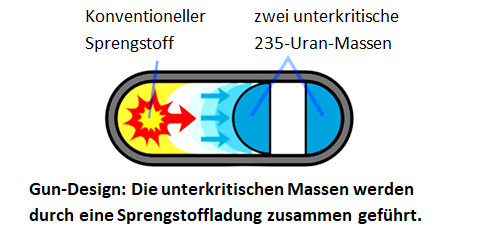
\includegraphics[scale=0.7]{Gun.png}
    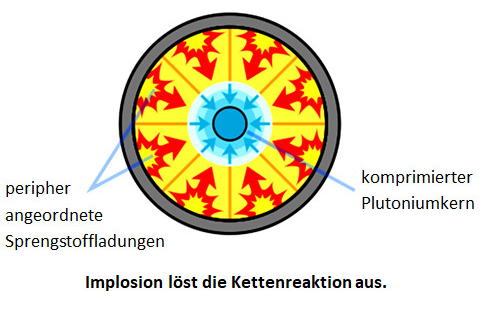
\includegraphics[scale=0.7]{Implosion.png}
\end{wrapfigure}

\textbf{Gun-Design:}
Das Gun-Design ist die einfachere der beiden Methoden und wurde bei der Hiroshima-Bombe (Little Boy) eingesetzt. Die Funktionsweise basiert darauf, 
zwei unterkritische Massen aus Uran-235 schnell zusammenzuführen (Z.b. mit TNT), um die kritische Masse zu überschreiten und die Kettenreaktion auszulösen. \hyperlink{gun_section}{Erklärung gibts auf Seite 4.}

\vspace*{2cm}

\noindent\textbf{Implosions-Design:}
Das Implosions-Design wurde bei der Nagasaki-Bombe (Fat Man) verwendet und ist deutlich komplexer als das Gun-Design. Es kommt bei Bomben zum Einsatz, die Plutonium-239 als spaltbares Material nutzen. 
Plutonium neigt bei zu langsamer Kompression zu vorzeitiger Zündung, was die Verwendung des Gun-Designs unmöglich macht. \hyperlink{implosion_section}{Erklärung gibts auf Seite 4.}

\newpage

\section{Funktion}
\hypertarget{implosion_section}{}
\hypertarget{gun_section}{}

\newpage

\section{Links}
\begin{center}
\qrcode{https://github.com/Jason4225/Latex}
\end{center}
\bigskip

\href{https://github.com/Tim-foe}{Github: Tim} \hspace{4cm}
\href{https://github.com/YoOlli}{Github: Olli} \hspace{4cm}
\href{https://github.com/Jason4225}{Github: J. Z.}

%\bibliographystyle{plain}
%\bibliography{bibliography.bib}

\end{document}